\section{Primeros pasos}

Uno de los campos en los cuales se hace m�s hincapi� dentro de la recuperaci�n
de informaci�n es el an�lisis, tanto sint�ctico como sem�ntico, de textos para
posteriormente poder analizar los resultados obtenidos y, por ejemplo, poder
buscar palabras que representen a una serie de documentos.

La construcci�n de analizadores de lenguaje natural es una tarea, que, adem�s
de ser compleja, el propio an�lisis tiene un conste computacional muy elevado
que fuerza al investigador a tener que utilizar equipos de alto rendimiento
para obtener resultados en un tiempo razonable.

El objetivo de este proyecto es la elaboraci�n de un envoltorio
(\textit{wrapper}) de uno de los analizadores m�s conocidos, el Stanford
Parser. Con �ste envoltorio se pretende hacer que el manejo del mismo sea lo
m�s sencillo posible, para que, la persona que lo use, se pueda abstraer
totalmente del funcionamiento interno del software y poder analizar documentos
f�cilmente.

\begin{figure}[h]
\begin{center}
	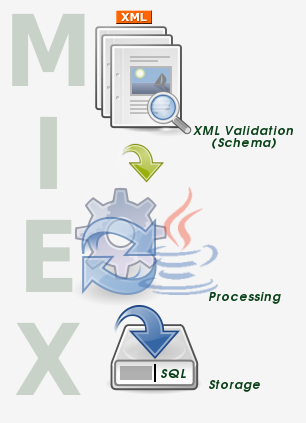
\includegraphics[bb=0 0 148 240]{images/miex.png}
	% miex.png: 257x416 pixel, 125dpi, 5.22x8.45 cm, bb=0 0 148 240
\end{center}
\caption{Esquema de funcionamiento de MIEX}
\end{figure} 



